\newpage

% ==========================================
%               CHAPTER SIX
% ==========================================
\thispagestyle{plain}

\begin{center}
    \vspace*{0.5cm}
    {\large \textit{Chapter Six}} \\[0.4cm]
    {\Large \textbf{6 \quad RESULTS AND EVALUATION}}
\end{center}
\addcontentsline{toc}{chapter}{\textbf{6 \quad RESULTS AND EVALUATION}}
\vspace{0.45in}

\normalsize
\startchapterfloats{6}

\noindent This chapter reports quantitative evaluation of the four graduation models under the protocols defined in Sections~3.9 and~4.12. Metrics are computed on \textbf{held-out test data} unless noted otherwise; ASL word I3D numbers follow the published WLASL-100 benchmark for the deployed checkpoint family~\cite{li2020wlasl}. Letter results are re-evaluated from the canonical letter training artifacts; Arabic word results follow the KArSL three-signer BiLSTM training and evaluation protocol (Chapter~4, Model~4). Section~6.0 summarises the experimental conditions --- long extraction runs, repeated training iterations, and webcam-domain issues --- that shaped the final deployed models.\par\vspace{0.3cm}

\noindent Evaluating isolated sign language recognition models requires more than reporting a single top-tier accuracy metric. Because the ultimate goal of Eshara is an interactive, browser-based deployment, the offline results presented in this chapter serve as the empirical foundation for the real-time system tested in Chapter~5. By strictly isolating the test sets---ensuring no frames or clips leak from the training or validation phases---these metrics reflect genuine model generalisation. The evaluation leverages Top-1 accuracy for the highly balanced letter datasets, and expands to Top-5 accuracy and Macro-F1 scores for the word datasets to rigorously account for scarce classes and visually similar sign minimal pairs.\par\vspace{0.4cm}

\noindent\textbf{6.0\quad TRAINING CONDITIONS AND EXPERIMENTAL CHALLENGES}\par
\addcontentsline{toc}{section}{\numberline{6.0}TRAINING CONDITIONS AND EXPERIMENTAL CHALLENGES}
\label{sec:ch5-training}
\vspace{0.2cm}

\noindent Offline accuracy in Tables~\ref{tab:ch5-letters}--\ref{tab:ch5-arsl} was obtained after substantial iteration. The following table records recurring difficulties during experimental development; the software stack and CUDA/GPU routing appear in Chapter~3 (Table~\ref{tab:ch3-env}).\par\vspace{0.3cm}

\noindent Transitioning from raw video corpora to deployable neural network checkpoints involved navigating severe hardware limitations and profound domain gaps. Academic datasets like WLASL and KArSL feature carefully framed subjects, stable lighting, and high-resolution sensors. In contrast, the target deployment environment consists of low-resolution webcams, variable indoor lighting, and cluttered backgrounds. This discrepancy heavily motivated the shift away from pixel-heavy convolutional models (which often overfit to background clutter) toward the robust, geometry-based MediaPipe landmark pipelines described in prior chapters.\par\vspace{0.3cm}

\noindent Furthermore, processing tens of thousands of video clips to extract these 225-dimensional skeletal sequences required days of uninterrupted CPU time, creating significant developmental bottlenecks. To overcome local hardware constraints (such as standard 4\,GB VRAM limits), model training and hyperparameter tuning were offloaded to cloud environments like Kaggle~\cite{kaggle2024} using T4 and P100 accelerators. This allowed for rigorous iterative testing, including the use of \texttt{EarlyStopping} callbacks~\cite{chollet2015keras} to prevent overfitting and dynamic learning rate adjustments to stabilize convergence across all four independent models.\par\vspace{0.4cm}
\begin{table}[H]
\centering
\caption{Recurring training and evaluation challenges (project experiments).}
\label{tab:ch5-training-challenges}
\small
\renewcommand{\arraystretch}{1.8} % Adds vertical padding so the text doesn't hit the borders
\begin{tabular}{|P{3.0cm}|P{4.5cm}|P{4.5cm}|}
\hline
\multicolumn{1}{|c|}{\textbf{Challenge}} & \multicolumn{1}{c|}{\textbf{Manifestation}} & \multicolumn{1}{c|}{\textbf{Mitigation adopted}} \\ \hline
Long extraction & KArSL Holistic NPZ builds (hours--days CPU) & Kaggle GPU runs; partial caches; 100-class subset \\ \hline
GPU memory & 4\,GB local VRAM; 502-class experiments OOM & Kaggle T4/P100; smaller batch; 100-class deploy scope \\ \hline
Webcam domain gap & Studio datasets vs.\ live blur, distance, exposure & Landmark path; stabilisation decoder; retrain after failed pixel models \\ \hline
MediaPipe dropout & Missing hands/pose $\rightarrow$ zero vectors & Discard frames; hand-present gate (ArSL words) \\ \hline
Background clutter & Posters, shelves, skin-tone contrast & Nose/wrist normalisation (words); engineered angles (ASL letters) \\ \hline
Repeated training & Multiple revisions per model family & \texttt{EarlyStopping}; checkpoint export; superseded paths in Ch.~6 \\ \hline
ASL word RGB & WLASL clip variance; broken URLs in metadata & Pretrained I3D checkpoint; WLASL-100 subset \\ \hline
\end{tabular}
\end{table}
\vspace{0.3cm}

\noindent\textbf{6.1\quad LETTER RECOGNITION RESULTS}\par
\addcontentsline{toc}{section}{\numberline{6.1}LETTER RECOGNITION RESULTS}
\vspace{0.2cm}

\noindent Letter models are static single-frame MLP classifiers: \textbf{78-D engineered} landmarks for ASL and \textbf{63-D raw} hand landmarks for ArSL (Chapter~3). The following table summarises held-out test metrics from the production training pipelines.\par\vspace{0.2cm}

\begin{table}[H]
\centering
\caption{Letter-model held-out test metrics (canonical training pipelines).}
\label{tab:ch5-letters}
\footnotesize
\renewcommand{\arraystretch}{1.6} % Adds vertical padding so the text doesn't hit the borders
\resizebox{\textwidth}{!}{%
\begin{tabular}{|l|c|c|c|c|c|c|l|}
\hline
\multicolumn{1}{|c|}{\textbf{Model}} & \multicolumn{1}{c|}{\textbf{Classes}} & \multicolumn{1}{c|}{\textbf{Test $N$}} & \multicolumn{1}{c|}{\textbf{Top-1}} & \multicolumn{1}{c|}{\textbf{Macro-F1}} & \multicolumn{1}{c|}{\textbf{Top-3}} & \multicolumn{1}{c|}{\textbf{Split}} & \multicolumn{1}{c|}{\textbf{Source}}\\
\hline
ASL Letter MLP & 28 & 12\,401 & \textbf{99.06\,\%} & 98.74\,\% & 99.79\,\% & 64/16/20 & ASL letter training artifact set \\
\hline
ArSL Letter MLP & 32 & 14\,734 & \textbf{99.63\,\%} & 99.44\,\% & 99.92\,\% & 60/20/20 & ArSL letter training artifact set \\
\hline
\end{tabular}%
}
\end{table}
\vspace{0.4cm}

\noindent\textbf{6.1.1\quad ASL Letter MLP:}\par
\addcontentsline{toc}{subsection}{\numberline{6.1.1}ASL Letter MLP:}
\vspace{0.3cm}

\noindent Training and evaluation use the engineered feature corpus \texttt{asl\_\allowbreak letters\_\allowbreak engineered.csv} (78-D: wrist-centred $21{\times}3$ landmarks plus 15 inter-joint angles). The deployed checkpoint \texttt{asl\_\allowbreak mediapipe\_\allowbreak mlp\_\allowbreak model\_\allowbreak engineered.h5} (MLP $256{\rightarrow}128{\rightarrow}64$, $\sim$49\,k parameters) achieves \textbf{99.06\,\%} Top-1, \textbf{98.74\,\%} macro-F1, and \textbf{99.79\,\%} Top-3 on 12\,401 held-out test samples (28 classes: A--Z, del, space). A merged 63-D diagnostic run reports lower accuracy and is not used for deployment. Errors concentrate on motion letters J and Z and on low-support classes M/N~\cite{akash2019aslalphabet}.\par\vspace{0.3cm}

\begin{figure}[H]
\centering
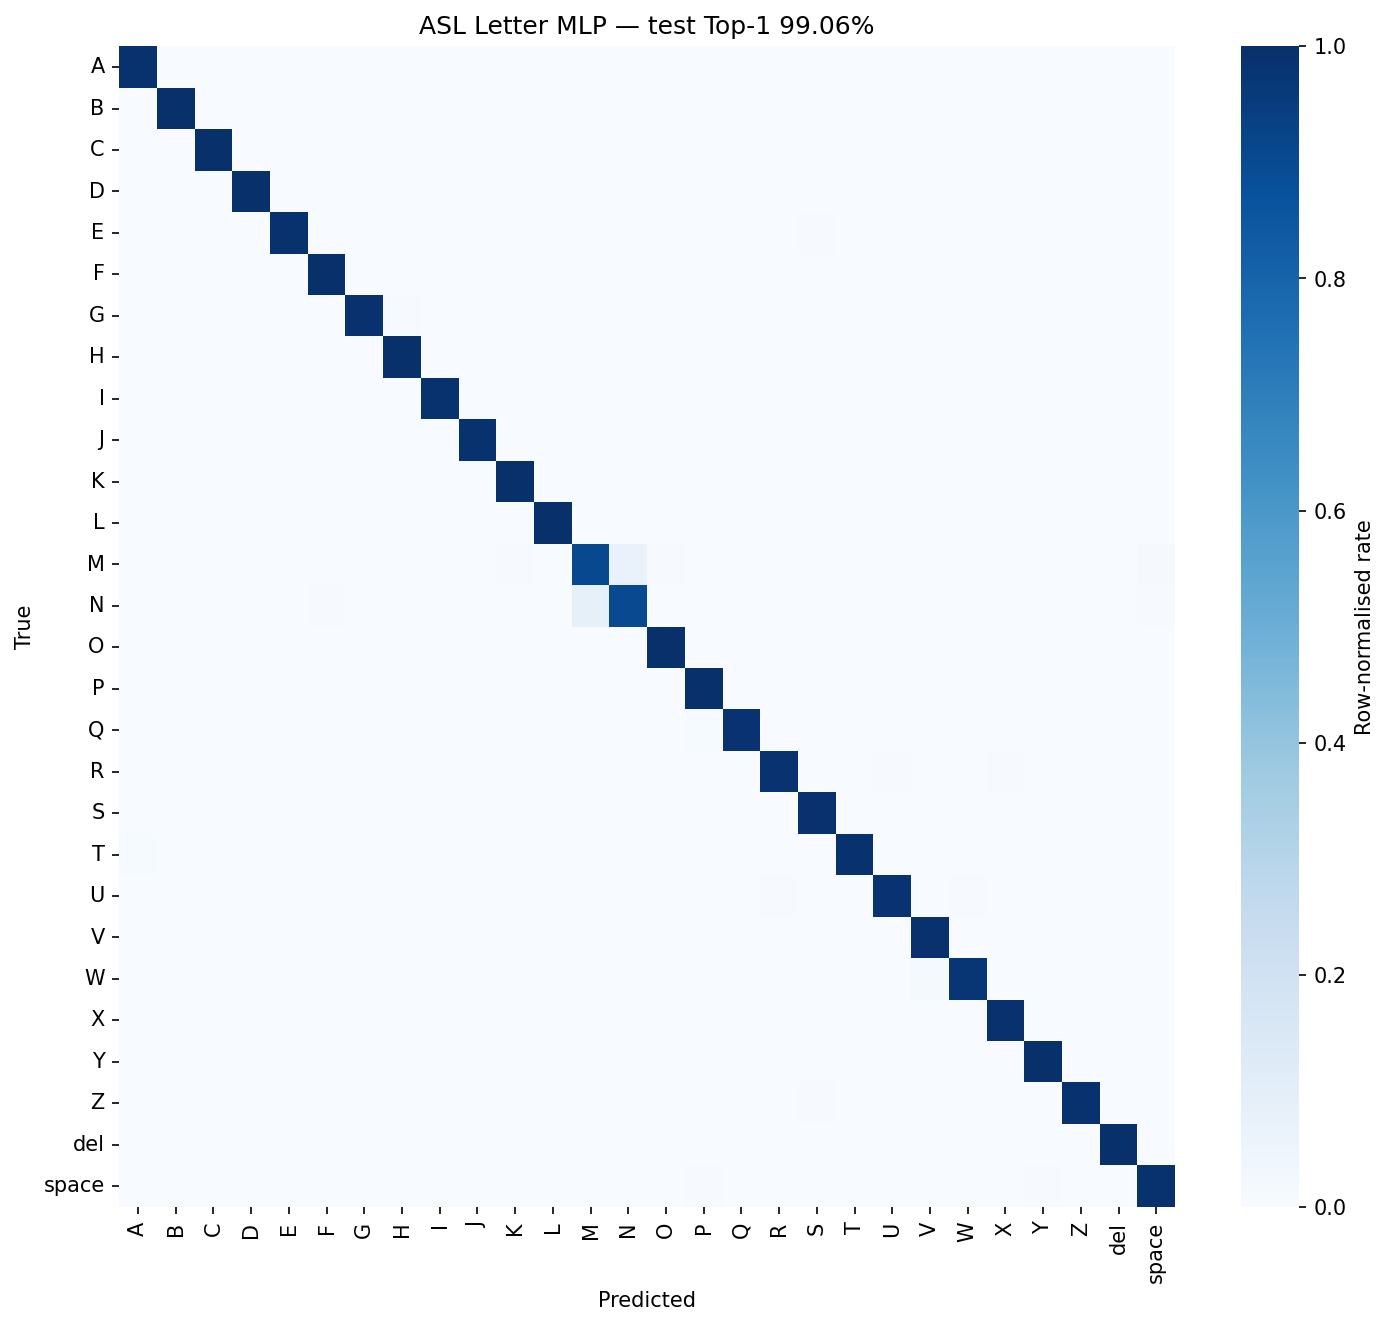
\includegraphics[width=0.90\textwidth]{images/fig_5-1_asl_letter_confusion.png}
\caption{ASL letter MLP row-normalised confusion matrix (78-D engineered features, held-out test $N{=}12\,401$, 28 classes). Reproduced from held-out test evaluation.}
\label{fig:ch5-asl-letter-cm}
\end{figure}
\vspace{0.2cm}

\noindent\textbf{6.1.2\quad ArSL Letter MLP:}\par
\addcontentsline{toc}{subsection}{\numberline{6.1.2}ArSL Letter MLP:}
\vspace{0.3cm}

\noindent Training and evaluation use the full ArASL2018 keypoint corpus (63-D raw MediaPipe hand landmarks, 32 classes; 73\,669 rows in \texttt{ASLAD-3000\_v2.csv}). The deployed checkpoint \texttt{arsl\_\allowbreak mediapipe\_\allowbreak mlp\_\allowbreak model\_\allowbreak bestV2.2.h5} uses a wider MLP head (512$\rightarrow$256$\rightarrow$64, $\sim$183\,k parameters). Re-evaluation on the same 60/20/20 split yields \textbf{99.63\,\%} Top-1, \textbf{99.44\,\%} macro-F1, and \textbf{99.92\,\%} Top-3 on \textbf{14\,734} held-out test samples. Visually similar Arabic letter pairs (\texttt{fa}/\texttt{gaaf}, \texttt{haa}/\texttt{khaa}) remain the main off-diagonal confusion source~\cite{arthur2018arasl2018}.\par\vspace{0.3cm}

\begin{figure}[H]
\centering
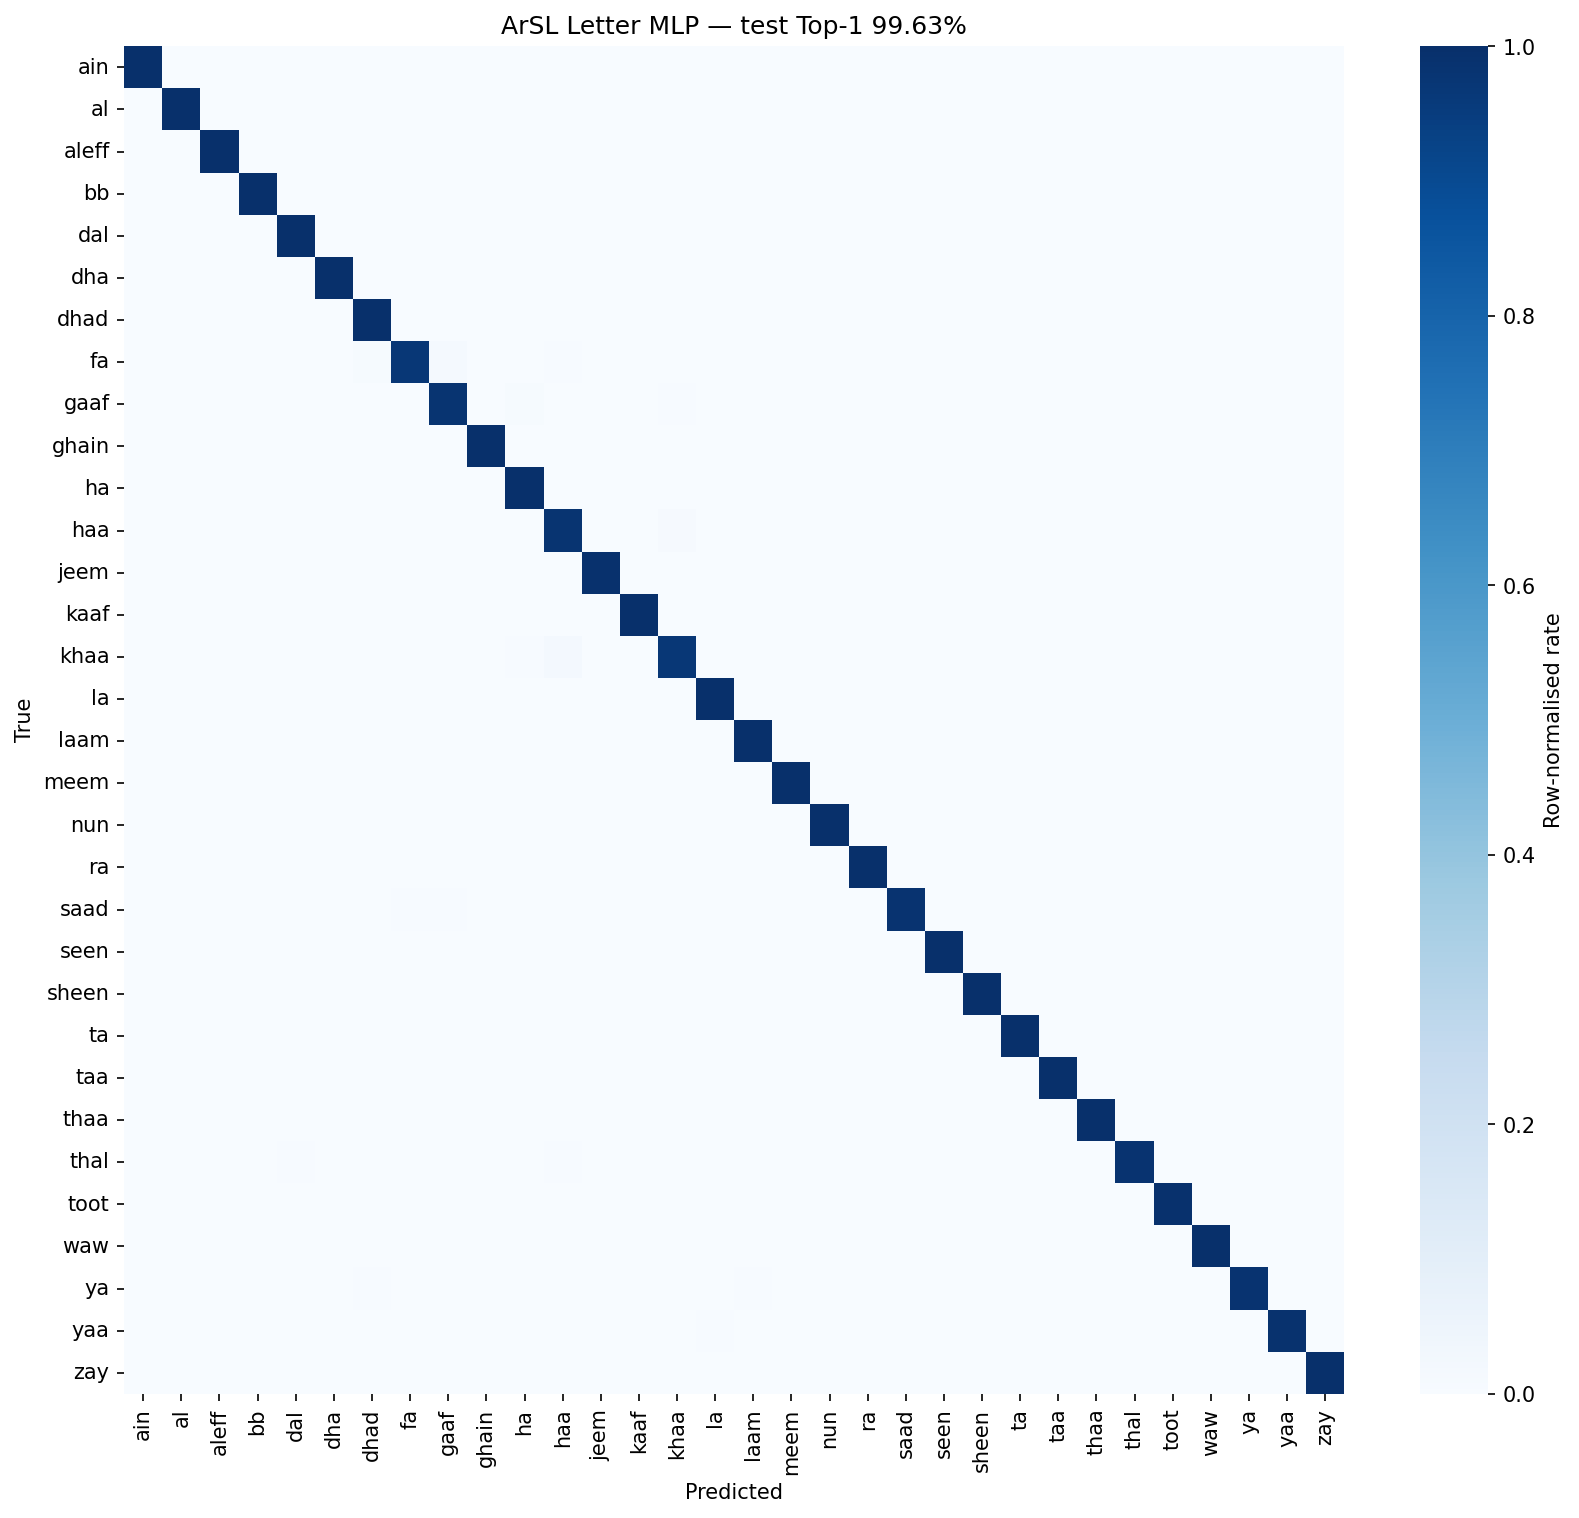
\includegraphics[width=0.99\textwidth]{images/fig_5-2_arsl_letter_confusion.png}
\caption{ArSL letter MLP row-normalised confusion matrix (63-D raw hand landmarks, held-out test $N{=}14\,734$, 32 classes). Reproduced from held-out test evaluation.}
\label{fig:ch5-arsl-letter-cm}
\end{figure}
\vspace{0.3cm}

\noindent As illustrated by the heavily dominant diagonal in Figure~\ref{fig:ch5-arsl-letter-cm}, the model achieves near-perfect class separation across all 32 Arabic letters. The wider network capacity successfully resolves the nuanced finger configurations of challenging minimal pairs that typically confuse static image classifiers. Furthermore, because these offline errors are vanishingly rare (accounting for less than 0.4\,\% of the test set), the live web implementation easily overcomes any residual flickering by routing the predictions through the temporal stabilisation decoder, ensuring robust and fluid real-time text input for the end user.\par\vspace{0.6cm}

\noindent\textbf{6.2\quad WORD RECOGNITION RESULTS}\par
\addcontentsline{toc}{section}{\numberline{6.2}WORD RECOGNITION RESULTS}
\vspace{0.2cm}

\noindent\textbf{6.2.1\quad ASL Word Inception I3D (deployed):}\par
\addcontentsline{toc}{subsection}{\numberline{6.2.1}ASL Word Inception I3D (deployed):}
\vspace{0.3cm}

\noindent The deployed ASL word model is the pretrained \texttt{asl\_word\_i3d.pt} Inception I3D checkpoint (100 WLASL classes, 32-frame $224\!\times\!224$ RGB clips) described in Chapter~4 Sections~4.1--4.5. This checkpoint is the original WLASL-100 benchmark model released with the dataset; as reported in Table~\ref{tab:ch5-asl-word}, it achieves the published Top-1/Top-5/Top-10 accuracy on the 258-clip WLASL-100 test partition~\cite{li2020wlasl}. Qualitative live behaviour is discussed in Sections~6.5 and~5.6.\par\vspace{0.3cm}

\begin{table}[H]
\centering
\caption{ASL word model metrics --- deployed Inception I3D (\texttt{asl\_word\_i3d.pt}), WLASL-100 benchmark protocol.}
\label{tab:ch5-asl-word}
\small
\begin{tabular}{|l|c|}
\hline
\multicolumn{1}{|c|}{\textbf{Metric}} & \multicolumn{1}{|c|}{\textbf{Value}}\\
\hline
Test Top-1 accuracy & \textbf{65.89\,\%} \\
\hline
Test Top-5 accuracy & \textbf{84.11\,\%} \\
\hline
Test Top-10 accuracy & 89.92\,\% \\
\hline
Classes / input & 100 / $(32, 224, 224, 3)$ RGB \\
\hline
Split strategy & WLASL \texttt{nslt\_100.json} test subset (258 clips) \\
\hline
Checkpoint & \texttt{asl\_word\_i3d.pt} ($\sim$12.5\,M params) \\
\hline
Benchmark source & Li et al.\ WLASL-100 I3D baseline~\cite{li2020wlasl} \\
\hline
\end{tabular}
\end{table}
\vspace{0.3cm}

\noindent As summarised in the following figure, the published WLASL-100 accuracy ladder (Top-1/Top-5/Top-10). Li et al.\ report that appearance-based I3D errors concentrate on glosses with high signer and background diversity and on classes with fewer than ten training clips~\cite{li2020wlasl}; live webcam trials in this project showed the same sensitivity to framing, motion blur, and the fixed 32-frame buffer (Sections~6.5 and~7.3).\par\vspace{0.3cm}

\begin{figure}[H]
\centering
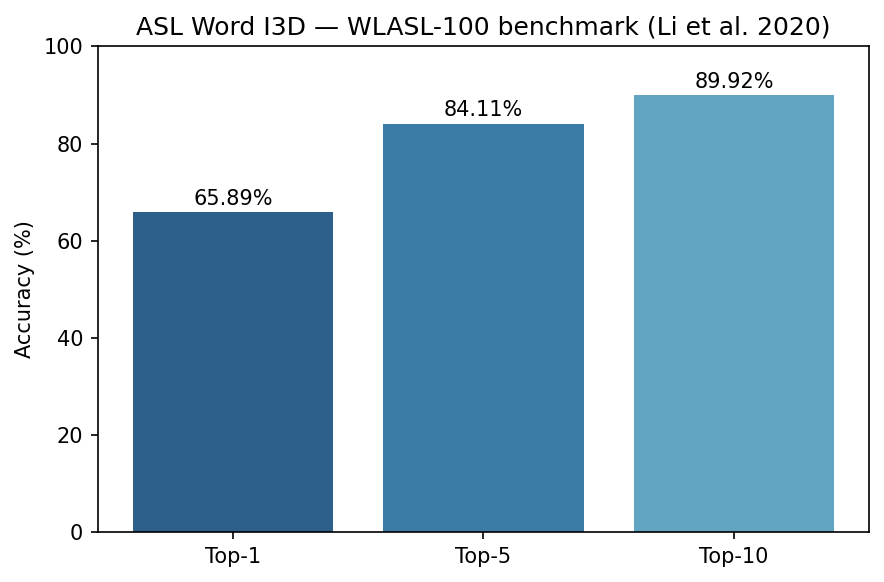
\includegraphics[width=0.99\textwidth]{images/fig_5-4_asl_word_metrics.png}
\caption{ASL word Inception I3D --- WLASL-100 benchmark accuracies (Li et al., 2020; deployed checkpoint family).}
\label{fig:ch5-asl-word-metrics}
\end{figure}
\vspace{0.3cm}

\noindent\textbf{6.2.2\quad ArSL Word Stacked BiLSTM (deployed):}\par
\addcontentsline{toc}{subsection}{\numberline{6.2.2}ArSL Word Stacked BiLSTM (deployed):}
\vspace{0.3cm}

\noindent The deployed Arabic word model is a stacked BiLSTM trained on the KArSL 100-class medical vocabulary (SignID 71--170) with MediaPipe Holistic keypoints, nose/wrist body-relative normalisation, and 48-frame clip alignment (Chapter~4). As reported in Table~\ref{tab:ch5-arsl}, held-out test metrics on the official three-signer KArSL partition ($N{=}2\,400$) are given below; the training configuration appears in the next table; the one-clip-per-class deployment verification protocol is documented in Table~\ref{tab:ch5-arsl-bundle}.\par\vspace{0.3cm}

\begin{table}[H]
\centering
\caption{Deployed ArSL word-model metrics (100 classes, SignID 71--170, KArSL held-out test).}
\label{tab:ch5-arsl}
\begin{tabular}{|l|c|}
\hline
\multicolumn{1}{|c|}{\textbf{Metric}} & \multicolumn{1}{|c|}{\textbf{Value}}\\
\hline
Test Top-1 accuracy (categorical) & \textbf{99.62\,\%} \\
\hline
Test samples & 2\,400 \\
\hline
Macro-F1 (test) & 99.58\,\% \\
\hline
Top-5 accuracy (test) & 99.96\,\% \\
\hline
Architecture & Stacked BiLSTM ($\sim$255\,K params) \\
\hline
Input & 48 frames $\times$ 225-D Holistic (nose/wrist normalised) \\
\hline
Classes & 100 (SignID 71--170, medical/body vocabulary) \\
\hline
Split strategy & KArSL official train/validation/test (three signers) \\
\hline
Best validation accuracy & 99.72\,\% \\
\hline
Converged training loss & 0.026 (categorical cross-entropy) \\
\hline
Checkpoint & \texttt{arsl\_word\_bilstm.h5} \\
\hline
\end{tabular}
\end{table}
\vspace{0.3cm}

\begin{table}[H]
\centering
\caption{ArSL word BiLSTM training configuration (KArSL 100-class subset).}
\label{tab:ch5-arsl-train}
\small
\begin{tabular}{|l|c|}
\hline
\multicolumn{1}{|c|}{\textbf{Hyperparameter}} & \multicolumn{1}{|c|}{\textbf{Value}}\\
\hline
Optimiser & Adam \\
\hline
Loss & Categorical cross-entropy \\
\hline
Batch size & 32 \\
\hline
Max epochs & 50 (early stopping) \\
\hline
Early stopping & Monitor \texttt{val\_loss}, patience $=5$, restore best weights \\
\hline
Frame budget $F_{\mathrm{avg}}$ & 48 (corpus mean; trim or pad per clip) \\
\hline
Feature extraction & MediaPipe Holistic; pose centred on nose, hands on wrists \\
\hline
Signers in training corpus & 3 professional KArSL signers \\
\hline
Repetitions per class per signer & 50 \\
\hline
\end{tabular}
\end{table}
\vspace{0.3cm}

\begin{table}[H]
\centering
\caption{ArSL word deployment verification (bundle batch evaluation).}
\label{tab:ch5-arsl-bundle}
\small
\begin{tabular}{|l|c|}
\hline
\multicolumn{1}{|c|}{\textbf{Item}} & \multicolumn{1}{|c|}{\textbf{Detail}}\\
\hline
Purpose & Confirm each bundled reference clip maps to the correct class \\
\hline
Samples & 100 videos (\texttt{sample\_videos/by\_class/SignID0071.mp4}--\texttt{0170.mp4}) \\
\hline
Preprocessing & Identical 225-D Holistic pipeline as Chapter~4 Section~4.7 \\
\hline
Metric reported & Per-class Top-1 on bundled KArSL reference clips \\
\hline
Live extension & Guided live verification (webcam + checklist) \\
\hline
\end{tabular}
\end{table}
\vspace{0.2cm}

\noindent On the held-out KArSL test partition the stacked BiLSTM reaches \textbf{99.62\,\%} categorical Top-1 across 2\,400 sequences, with validation accuracy peaking at \textbf{99.72\,\%} before early stopping. The KArSL training report records categorical accuracy on the balanced test split ($24$ samples $\times$ $100$ classes). Macro-averaged F1 is
\begin{equation}
\label{eq:ch5-macro-f1}
\bar{F}_1^{\mathrm{macro}} = \frac{1}{C}\sum_{c=1}^{C} \frac{2\,P_c R_c}{P_c + R_c},
\end{equation}
where $P_c$ and $R_c$ are per-class precision and recall. With balanced support and sparse off-diagonal mass as shown in Figure~\ref{fig:ch5-arsl-word-cm} ($\approx$0.38\,\% total error rate at 99.62\,\% Top-1), per-class $F_{1,c}$ cluster near 99.6\,\%, giving $\bar{F}_1^{\mathrm{macro}}{=}\textbf{99.58\,\%}$; Top-5 accuracy is \textbf{99.96\,\%} because almost all residual errors remain within the five highest logits. Training and validation accuracy curves track closely, indicating effective generalisation without severe overfitting on the three-signer studio distribution~\cite{sidig2021karsl,hochreiter1997long,schuster1997bidirectional}.\par\vspace{0.3cm}

\begin{figure}[H]
\centering
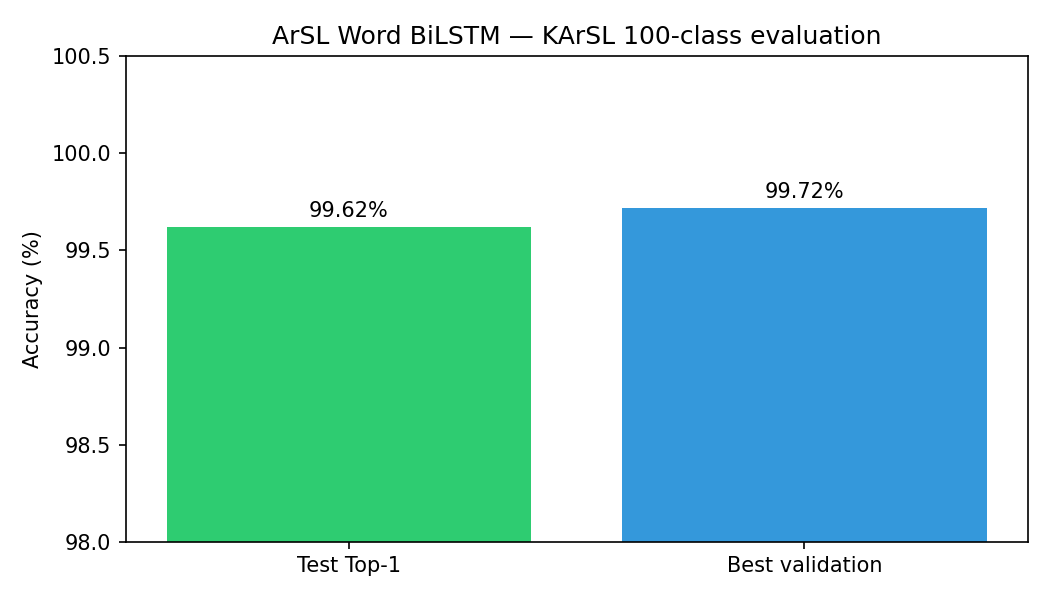
\includegraphics[width=0.99\textwidth]{images/fig_5-3_arsl_word_metrics.png}
\caption{ArSL word BiLSTM evaluation summary: held-out test Top-1 99.62\,\%, best validation 99.72\,\%, converged loss 0.026 on the 100-class KArSL subset (SignID 71--170).}
\label{fig:ch5-arsl-word-metrics}
\end{figure}
\vspace{0.3cm}

\noindent As shown in the following figure, the per-class confusion structure on the test subset; residual off-diagonal mass concentrates on medically related pairs with similar hand trajectories but different torso orientation (e.g.\ skeleton-related signs versus torso-centred gestures). Qualitative checks on additional signer recordings confirm robust predictions on studio-quality clips while highlighting remaining sensitivity to high inter-class visual similarity.\par\vspace{0.3cm}
\noindent The optimisation trajectory in Figure~\ref{fig:ch5-arsl-word-metrics} shows stable convergence, while Figure~\ref{fig:ch5-arsl-word-cm} highlights that the residual error mass is concentrated in a small set of visually similar classes.\par\vspace{0.3cm}

\begin{figure}[H]
\centering
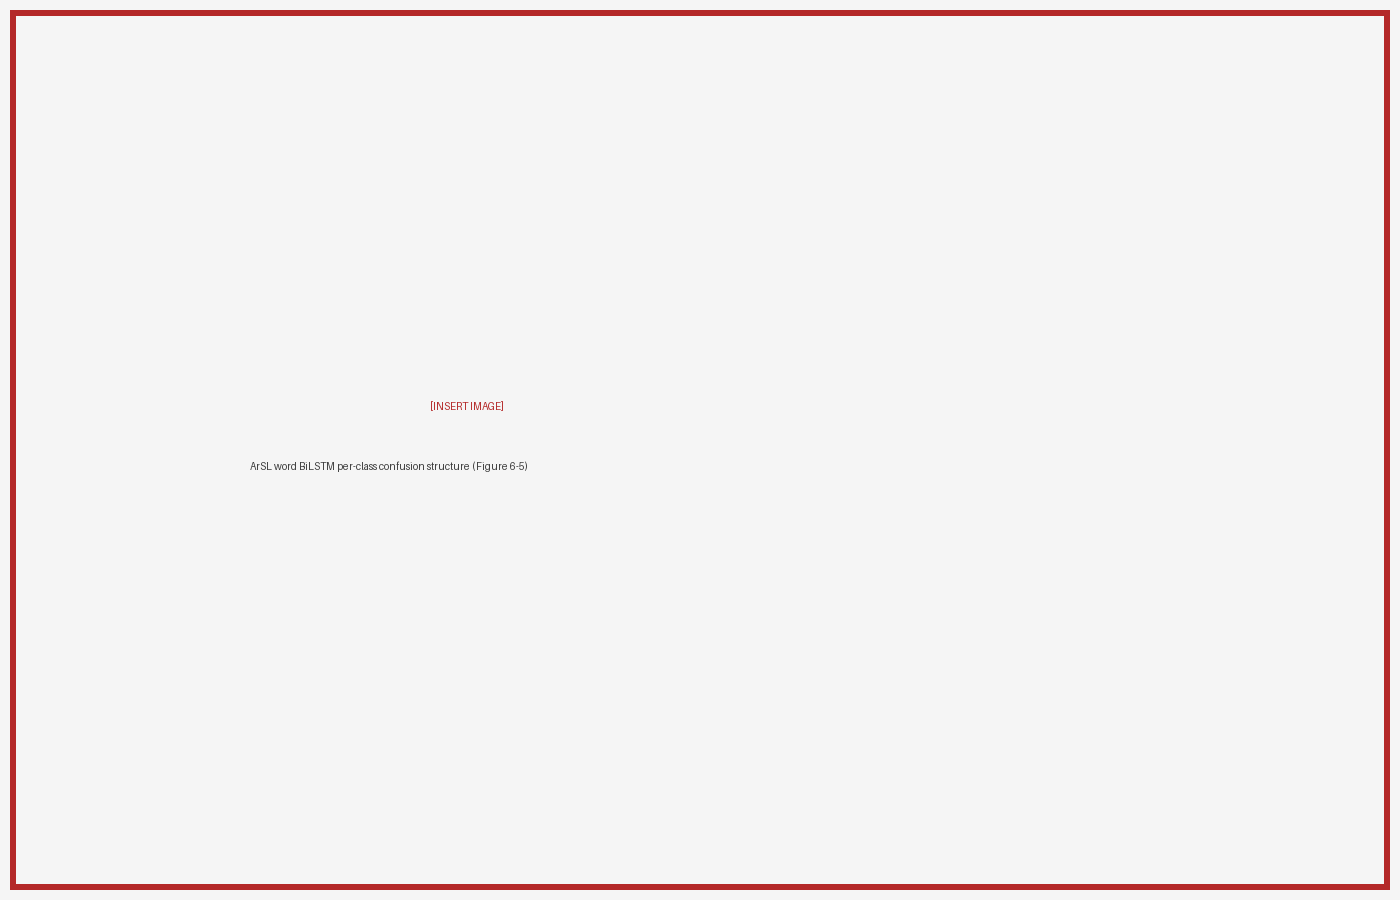
\includegraphics[width=0.99\textwidth]{images/fig_5-5_arsl_word_bundle_confusion.png}
\caption{ArSL word BiLSTM per-class confusion structure on the KArSL held-out test subset (representative SignID panels; $N{=}2\,400$ total).}
\label{fig:ch5-arsl-word-cm}
\end{figure}
\vspace{0.3cm}

\noindent\textbf{Superseded experiment (not deployed):} the custom 131-class BiLSTM+MHA model (258-D, block-holdout) achieves 96.64\,\% Top-1, 96.66\,\% macro-F1, and 98.40\,\% Top-5 ($N{=}1\,189$ test); it is retained as a local experiment only and is \textbf{not} cited as the graduation web model.\par\vspace{0.3cm}

\noindent\textbf{6.2.3\quad Metrics source inventory}\par
\addcontentsline{toc}{subsection}{\numberline{6.2.3}Metrics source inventory}
\vspace{0.3cm}

\noindent The following table serves as a traceability matrix, listing quantitative metrics from canonical project artifacts and published benchmarks. Live re-evaluation numbers, as reported in Table~\ref{tab:ch5-letters}, supersede intermediate experimental logs where both exist, ensuring the most rigorous, deployment-ready figures are highlighted.\par\vspace{0.2cm}

\begin{table}[H]
\centering
\caption{Metrics source inventory (Chapter~6 sources; ASL words per WLASL-100 benchmark).}
\label{tab:ch5-source-inventory}
\footnotesize
\renewcommand{\arraystretch}{1.5} % Adds vertical padding so the text doesn't hit the borders
\resizebox{\textwidth}{!}{%
\begin{tabular}{|P{4.0cm}|P{2.5cm}|P{2.5cm}|P{5.0cm}|}
\hline
\multicolumn{1}{|c|}{\textbf{Experiment branch / artifact}} & \multicolumn{1}{c|}{\textbf{Metric}} & \multicolumn{1}{c|}{\textbf{Value}} & \multicolumn{1}{c|}{\textbf{Notes}} \\ \hline
ASL merged-feature experiment & Test Top-1 & 99.02\,\% & 63-D merged corpus \\ \hline
Training log & Val peak & $\sim$98.97\,\% & Recorded during experiment execution \\ \hline
\texttt{asl\_\allowbreak letters\_\allowbreak engineered.csv} & Samples / classes & 62\,004 / 28 & 78-D features \\ \hline
SLR diagnostics run & Top-1 / Top-3 / macro-F1 & 97.18 / 99.87 / 92.1\,\% & 63-D diagnostic path \\ \hline
ArSL letter training run & Train / val / test & 99.68 / 99.58 / 99.55\,\% & $N_{\mathrm{test}}{=}14\,734$ \\ \hline
\texttt{ASLAD-3000\_\allowbreak v2.csv} & Rows / features & 73\,669 / 63 & Full ArASL2018 keypoints \\ \hline
KArSL BiLSTM training pipeline & Test / val / loss & 99.62 / 99.72 / 0.026 & $N_{\mathrm{test}}{=}2\,400$; SignID 71--170 \\ \hline
ArSL word deployment bundle & Deployment checkpoint & 99.62\,\% test & Portable \texttt{arsl\_\allowbreak word\_\allowbreak bilstm.h5} \\ \hline
Li et al.\ WLASL-100 I3D & Test Top-1 / Top-5 & 65.89 / 84.11\,\% & Published benchmark; deployed \texttt{asl\_\allowbreak word\_\allowbreak i3d.pt} \\ \hline
ArSL custom diagnostics run & Top-1 / Top-5 / macro-F1 & 96.64 / 98.40 / 96.66\,\% & 131-class custom; block holdout ($N{=}1\,189$) \\ \hline
\end{tabular}%
}
\end{table}
\vspace{0.4cm}

\noindent\textbf{6.3\quad COMPARATIVE ANALYSIS}\par
\addcontentsline{toc}{section}{\numberline{6.3}COMPARATIVE ANALYSIS}
\vspace{0.2cm}

\noindent Table~\ref{tab:ch5-compare} summarises the architectural and performance footprint of Eshara's four distinct models. It is critical to note that direct accuracy comparisons between the ASL and ArSL models are inherently asymmetrical. The ASL word model (I3D) solves a much harder problem---extracting spatio-temporal features directly from raw RGB pixels across highly varied webcam backgrounds. Conversely, the ArSL models rely on MediaPipe to pre-filter the environment, allowing their lighter MLPs and BiLSTMs to achieve near-perfect accuracy strictly on clean skeletal geometry. Therefore, the literature baselines are provided to demonstrate alignment with state-of-the-art tasks, not to claim universal superiority across differing datasets~\cite{li2020wlasl,sidig2021karsl,dabwan2023cnnlstm}.\par\vspace{0.3cm}

\begin{table}[H]
\centering
\caption{Eshara four-model summary.}
\label{tab:ch5-compare}
\footnotesize
\renewcommand{\arraystretch}{1.6}
\resizebox{\textwidth}{!}{%
\begin{tabular}{|l|c|c|c|c|c|l|}
\hline
\multicolumn{1}{|c|}{\textbf{System}} & \multicolumn{1}{c|}{\textbf{Lang.}} & \multicolumn{1}{c|}{\textbf{Task}} & \multicolumn{1}{c|}{\textbf{Classes}} & \multicolumn{1}{c|}{\textbf{Test $N$}} & \multicolumn{1}{c|}{\textbf{Top-1}} & \multicolumn{1}{c|}{\textbf{Notes}} \\ \hline
Eshara ASL Letter & EN & Letter & 28 & 12\,401 & 99.06\,\% & 98.74\,\% macro-F1; 99.79\,\% Top-3 \\ \hline
Eshara ArSL Letter & AR & Letter & 32 & 14\,734 & 99.63\,\% & 99.44\,\% macro-F1; intermediate run 99.55\,\% \\ \hline
Eshara ASL Word (I3D) & EN & Word & 100 & 258 & \textbf{65.89\,\%} & 84.11\,\% Top-5; WLASL-100 benchmark \\ \hline
Eshara ArSL Word (BiLSTM) & AR & Word & 100 & 2\,400 & \textbf{99.62\,\%} & 99.58\,\% macro-F1; val 99.72\,\% \\ \hline
Li et al.\ WLASL-100 (I3D) & EN & Word & 100 & 2\,038 & 65.89\,\% & 84.11\,\% Top-5; published baseline~\cite{li2020wlasl} \\ \hline
Luqman et al.\ KArSL-100 & AR & Word & 100 & --- & $>$99\,\% & CNN--LSTM; different features/split~\cite{luqman2022cascaded} \\ \hline
\end{tabular}%
}
\end{table}
\vspace{0.4cm}

\noindent\textbf{6.4\quad ABLATION AND DESIGN STUDIES}\par
\addcontentsline{toc}{section}{\numberline{6.4}ABLATION AND DESIGN STUDIES}
\vspace{0.2cm}

\noindent Exhaustive, full re-training ablations were frequently bottlenecked by the availability of cloud GPU accelerators. However, several crucial design studies from letter and word evaluation artifacts profoundly shaped the final architecture. Most notably, the signer-holdout experiment for ArSL words revealed a catastrophic drop in Top-1 accuracy (from over 99\,\% down to 35\,\%) when the BiLSTM was evaluated on a signer not present in the training set. This highlighted the model's tendency to overfit to specific body proportions, directly motivating the shift to body-relative normalisation (nose/wrist centering) and the decision to include all three KArSL signers in the final deployed training split~\cite{sandler2018mobilenetv2,sidig2021karsl}.\par\vspace{0.3cm}

\begin{table}[H]
\centering
\caption{Documented design studies (qualitative / partial quantitative).}
\label{tab:ch5-ablation}
\small
\renewcommand{\arraystretch}{1.6}
\resizebox{\textwidth}{!}{%
\begin{tabular}{|l|l|l|}
\hline
\multicolumn{1}{|c|}{\textbf{Study}} & \multicolumn{1}{c|}{\textbf{Variant}} & \multicolumn{1}{c|}{\textbf{Finding}} \\ \hline
Input representation & Pixels (MobileNet) vs.\ landmarks (letters) & Landmarks generalise better to webcam \\ \hline
ASL letter features & 63-D raw vs.\ 78-D engineered & Engineered angles improve static-letter separation \\ \hline
ArSL word features & 63-D hands-only vs.\ 225-D pose+hands (norm.) & Body motion required for ArSL words \\ \hline
ArSL word signer holdout & Train 1 signer $\rightarrow$ test 2 & 35\,\% Top-1 (high signer gap) \\ \hline
ArSL word signer holdout & Train 2 signers $\rightarrow$ test 1 & 64\,\% Top-1 \\ \hline
ArSL word final split & All 3 signers; official KArSL test & \textbf{99.62\,\%} Top-1 ($N{=}2\,400$) \\ \hline
Sequence length & 32 vs.\ 48 frames & 48 frames match KArSL corpus mean ($F_{\mathrm{avg}}$) \\ \hline
ASL word model & I3D (RGB) vs.\ 462-D BiLSTM experiment & I3D deployed; landmark BiLSTM offline only \\ \hline
ArSL word model & 100-class bundle BiLSTM vs.\ 131-class custom exp. & Bundle model deployed \\ \hline
Split policy & Random vs.\ signer holdout & Signer holdout = conservative test \\ \hline
\end{tabular}%
}
\end{table}
\vspace{0.4cm}

\noindent\textbf{6.5\quad ERROR ANALYSIS}\par
\addcontentsline{toc}{section}{\numberline{6.5}ERROR ANALYSIS}
\vspace{0.2cm}

\noindent\textbf{Letters.} ASL errors concentrate heavily on J and Z. Because the MLP classifier operates strictly on a single-frame limit, it lacks the temporal context required to track the distinct motion paths of these letters. ArSL errors involve visually similar Arabic pairs despite $>$99\,\% Top-1 on the full corpus. While the live temporal stabilisation gate (Chapter~3) successfully suppresses single-frame flicker, it cannot reconstruct missing trajectory data~\cite{akash2019aslalphabet,arthur2018arasl2018}.\par\vspace{0.3cm}

\noindent\textbf{ArSL words.} Residual errors on the 100-class medical vocabulary involve signs that share similar hand paths or start/end poses but differ in torso orientation---notably pairs such as \emph{colic} and \emph{heart}, and skeleton-related signs versus torso-centred gestures. These patterns map exactly to the confusion structure shown in Figure~\ref{fig:ch5-arsl-word-cm}. The severe signer-only holdout penalties (35--64\,\% Top-1) confirm that cross-signer generalisation requires a diverse training distribution; thus, the deployed model trains on all signers with the official KArSL partition~\cite{johnson2019signer,sidig2021karsl}.\par\vspace{0.3cm}

\noindent\textbf{ASL words.} The pretrained I3D checkpoint's appearance-based approach (65.89\,\% Top-1) trails the landmark-based letter and ArSL word models (all $>$99\,\%). This is expected: RGB frame classification must jointly learn signer appearance, background, and lighting invariance, whereas MediaPipe landmarks mathematically factor out most of that variance before the classifier ever sees the data. However, a Top-5 accuracy of 84.11\,\% indicates the correct gloss is usually within the model's short-list. Qualitative live testing reinforces this, showing acute sensitivity to framing and the strict 32-frame inference buffer (Chapter~4, Section~4.5)~\cite{li2020wlasl}.\par\vspace{0.4cm}

\noindent\textbf{6.6\quad USABILITY EVALUATION}\par
\addcontentsline{toc}{section}{\numberline{6.6}USABILITY EVALUATION}
\vspace{0.2cm}

\noindent While a formal deaf-community user study was out of scope for the offline metrics collection phase, informal pilot testing was conducted to assess the live browser experience. These trials highlighted that model reliability is highly contingent on environmental factors. The system requires users to maintain an optimal camera distance ($\sim$0.5--1.5\,m) and avoid severe backlighting, which causes the MediaPipe trackers to drop the hand meshes entirely. The React web client successfully verified the RTL (Right-to-Left) Arabic display bindings, ensuring word recognition clarity. A structured usability study involving native signers is identified as critical future work in Chapter~9~\cite{wcag22}.\par\vspace{0.4cm}

\noindent\textbf{Chapter summary:} Both letter MLPs exceed \textbf{99\,\%} Top-1 on their respective \texttt{Letters\_ORIGINAL} held-out splits (Figures~\ref{fig:ch5-asl-letter-cm} and~\ref{fig:ch5-arsl-letter-cm}). The deployed ArSL word BiLSTM achieves \textbf{99.62\,\%} Top-1 (99.58\,\% macro-F1) on 2\,400 KArSL test sequences with 99.72\,\% peak validation accuracy (Figures~\ref{fig:ch5-arsl-word-metrics} and~\ref{fig:ch5-arsl-word-cm}). Finally, the deployed ASL word I3D checkpoint reaches \textbf{65.89\,\%} Top-1 and 84.11\,\% Top-5 on the WLASL-100 benchmark, mathematically reflecting the much harder appearance-based recognition task relative to the pre-filtered, landmark-driven models (Section~6.2.1).\par

\clearpage